\documentclass[border=4pt,12pt]{standalone}
% House style for redrawn exam diagrams (diagram-v4: 0.4pt lines, filled -latex arrows, fine dashes; stipple and hatching drawn as real dots/lines (no PDF/SVG patterns, so they render in every browser and at any scale); transparent background). Every figure \input's this.
\usepackage{amsmath,amssymb}
\usepackage{txfonts}
\usepackage{pdfrender,xcolor}
% \halo{text}: label on shading. The shading stops just around each letter's outline (a thin knock-out that follows the
% glyphs, like the papers' typesetting), never a box. Owner: "I don't want a box around the text".
\newcommand{\halo}[1]{\leavevmode\rlap{\pdfrender{TextRenderingMode=2,LineWidth=2.2pt,LineJoinStyle=1,StrokeColor=white,FillColor=white}#1}#1}
\usepackage{tikz,pgfplots}
\pgfplotsset{compat=1.18}
\usetikzlibrary{arrows.meta,calc,angles,quotes,patterns,patterns.meta,intersections,positioning,decorations.markings,shapes.geometric}
% Stipple and hatching are drawn as actual dots / lines clipped to the region (path picture), NOT as pattern fills:
% SVG <pattern> fills vanish or blur when browsers scale the image, so the owner could not see the shading.
% Each dot is a 0.72pt square (keeps SVGs small; reads as a dot at print size). Dots sit on one global staggered grid, so neighbouring regions line up.
\makeatletter
\newdimen\ex@x \newdimen\ex@y \newdimen\ex@xa \newdimen\ex@ya \newdimen\ex@xb \newdimen\ex@yb \newcount\ex@row
\def\exam@stipplecolor{black!75}\def\exam@dotr{0.42pt}\def\exam@dotgap{2.5}
\def\ex@rowdots{\ifdim\ex@x<\ex@xb \pgfpathrectangle{\pgfqpoint{\dimexpr\ex@x-0.36pt\relax}{\dimexpr\ex@y-0.36pt\relax}}{\pgfqpoint{0.72pt}{0.72pt}}\advance\ex@x by \exam@dotgap pt\relax\expandafter\ex@rowdots\fi}
\def\exam@stipple{%
  \pgftransformreset% dots are sized in real points even inside scaled pictures
  \pgfpointanchor{path picture bounding box}{south west}\ex@xa=\pgf@x \ex@ya=\pgf@y
  \pgfpointanchor{path picture bounding box}{north east}\ex@xb=\pgf@x \ex@yb=\pgf@y
  \pgfsetfillcolor{\exam@stipplecolor}\pgfmathsetmacro\ex@h{\exam@dotgap/2}%
  \pgfmathtruncatemacro\ex@r{floor(\ex@ya/\ex@h)-1}\ex@row=\ex@r\relax
  \ex@y=\ex@r\dimexpr\ex@h pt\relax
  \loop\ifdim\ex@y<\ex@yb
    \pgfmathtruncatemacro\ex@c{floor(\ex@xa/\exam@dotgap)-1}\ex@x=\ex@c\dimexpr\exam@dotgap pt\relax
    \ifodd\ex@row \advance\ex@x by \ex@h pt\fi
    \ex@rowdots
    \advance\ex@y by \ex@h pt \advance\ex@row by 1
    \ifnum\numexpr\ex@row-(\ex@row/4)*4\relax=0 \pgfusepath{fill}\fi% flush every 4 rows: bounded TeX memory, few clip copies in the SVG
  \repeat\pgfusepath{fill}}
\newdimen\ex@d
\def\exam@hatch#1{% #1 = 1 for /, -1 for \ ; lines 45 degrees, 3pt apart
  \pgftransformreset
  \pgfpointanchor{path picture bounding box}{south west}\ex@xa=\pgf@x \ex@ya=\pgf@y
  \pgfpointanchor{path picture bounding box}{north east}\ex@xb=\pgf@x \ex@yb=\pgf@y
  \ex@d=\dimexpr\ex@yb-\ex@ya\relax \ex@x=\dimexpr\ex@xa-\ex@d\relax
  \loop\ifdim\ex@x<\ex@xb
    \ifnum#1>0 \pgfpathmoveto{\pgfqpoint{\ex@x}{\ex@ya}}\pgfpathlineto{\pgfqpoint{\dimexpr\ex@x+\ex@d\relax}{\ex@yb}}%
    \else \pgfpathmoveto{\pgfqpoint{\ex@x}{\ex@yb}}\pgfpathlineto{\pgfqpoint{\dimexpr\ex@x+\ex@d\relax}{\ex@ya}}\fi
    \advance\ex@x by 4.24pt
  \repeat
  \pgfsetlinewidth{0.4pt}\pgfsetstrokecolor{black}\pgfusepath{stroke}}
\def\examstipple{\exam@stipple}\def\examhatch{\exam@hatch}\def\examsetstipplecolor#1{\def\exam@stipplecolor{#1}}\def\examsetdotgap#1{\def\exam@dotgap{#1}}
\makeatother
% (legacy pattern kept for old files)
% staggered stipple like the NESA papers' dotted shading
\pgfdeclarepatternformonly{exam stipple}{\pgfpointorigin}{\pgfqpoint{2.2pt}{2.2pt}}{\pgfqpoint{2.2pt}{2.2pt}}{%
  \pgfpathcircle{\pgfqpoint{0.55pt}{0.55pt}}{0.42pt}\pgfpathcircle{\pgfqpoint{1.65pt}{1.65pt}}{0.42pt}\pgfusepath{fill}}
\tikzset{
  every picture/.style={line width=0.6pt, >={Latex[length=2mm,width=1.3mm]}},
  curve/.style={line width=0.6pt},
  open arrow/.style={-{Latex[length=2mm,width=1.3mm]}},  % owner: filled -latex heads everywhere, no open chevrons
  aux/.style={dash pattern=on 2pt off 1.5pt, line width=0.6pt},
  shade/.code={\def\exA{#1}\def\exB{none}\ifx\exA\exB\else\pgfkeysalso{fill=black!18}\fi},
  shade/.default=on,
  shade dots/.style={fill=none, path picture={\examstipple}},
  stipple color/.code={\examsetstipplecolor{#1}},
  stipple gap/.code={\examsetdotgap{#1}},
  shade dense dots/.style={fill=none, stipple gap=1.6, path picture={\examstipple}},
  shade hatch/.style={fill=none, path picture={\examhatch{1}}},
  shade hatch reverse/.style={fill=none, path picture={\examhatch{-1}}},
  shade solid/.style={fill=black},
  pt/.style={circle, fill, inner sep=1.1pt},
  open pt/.style={circle, draw, fill=white, inner sep=1.1pt},
}
\pgfplotsset{
  exam axes/.style={axis lines=middle, axis line style={->}, xlabel={$x$}, ylabel={$y$},
    xlabel style={anchor=west}, ylabel style={anchor=south}, tick label style={font=\small},
    every axis plot/.append style={line width=0.6pt, black}, samples=200, clip=false,
    enlargelimits=false, axis on top},
}

\begin{document}
% 2025 NESA HSC Q23 solution: females and males normal curves; males' upper tail beyond x shaded, bar marks <2.5% of females (crop pixels, y down; curves traced)
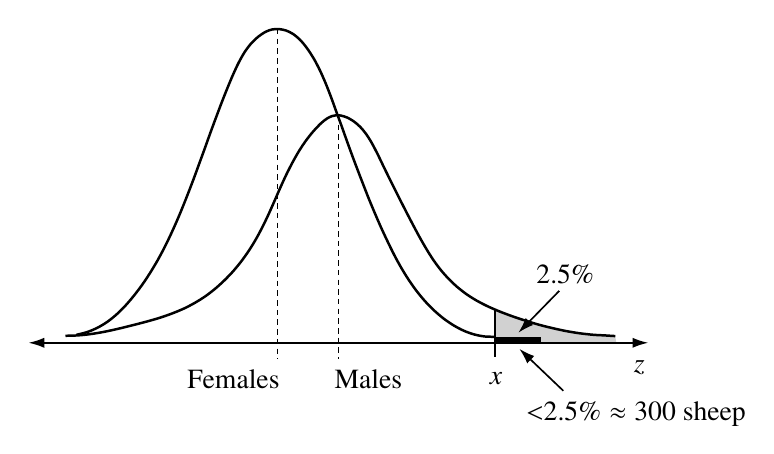
\begin{tikzpicture}[x=0.0127cm,y=-0.0127cm]
  \fill[shade] (477,327) -- (477,293.8) -- plot[smooth] coordinates {(479,294.5) (480.4,295.2) (481.8,295.9) (483.2,296.5) (484.7,297.2) (486.2,297.8) (487.8,298.4) (489.4,299) (491.1,299.6) (492.7,300.2) (494.4,300.8) (496,301.4) (497.7,301.9) (499.3,302.5) (500.9,303) (502.5,303.5) (504.1,304) (505.8,304.5) (507.4,305) (509.1,305.5) (510.8,306) (512.5,306.4) (514.2,306.9) (515.9,307.4) (517.6,307.9) (519.3,308.4) (520.9,308.9) (522.6,309.4) (524.3,309.8) (526,310.3) (527.6,310.7) (529.3,311.1) (531,311.6) (532.6,312) (534.3,312.3) (536,312.7) (537.6,313.1) (539.3,313.4) (541.1,313.8) (542.7,314.1) (544.4,314.5) (546.1,314.8) (547.8,315.2) (549.5,315.6) (551.1,315.9) (552.7,316.2) (554.3,316.4) (556.1,316.7) (557.8,316.9) (559.4,317.2) (561.1,317.5) (562.8,317.8) (564.5,318.1) (566.1,318.4) (567.7,318.7) (569.2,318.8) (570.7,319) (572.2,319) (573.6,319.1) (575,319) (586,319.6) (597,320.3)} -- (598,327) -- cycle;
  \fill (477,321) rectangle (523,328);
  \draw[<->] (10,327) -- (630,327);
  \draw[line width=0.9pt] plot[smooth]coordinates {(58,319) (68.36,316.4) (78.68,312.1) (88.48,306.3) (97.79,298.9) (106.8,290) (115.6,279.7) (123.9,268.7) (131.8,256.8) (139.1,244.6) (146,231.7) (152.4,218.5) (158.6,204.7) (164.4,190.8) (170.1,176.4) (175.6,162) (181,147.2) (186.4,132.4) (191.8,117.3) (197.2,102.7) (202.7,88.08) (208.3,73.88) (214.2,59.73) (220.1,47.03) (226.1,36.36) (232.7,27.6) (240,20.65) (247.4,15.79) (253.9,13.53) (260.7,13.17) (267.9,14.69) (274.7,18.12) (281.6,23.83) (288.4,32.01) (295.4,42.74) (301.5,54.39) (307.2,67.25) (312.6,81.06) (317.9,95.7) (323.4,110.7) (328.7,125.6) (334.1,140.4) (339.6,155) (345.2,169.5) (350.9,184) (356.8,198.1) (362.9,212.1) (369.4,226) (375.9,239.2) (382.9,252) (390.2,263.8) (398.1,275) (406.5,285.2) (415.6,294.5) (425.2,302.7) (435.3,309.6) (445.6,315) (456,318.7) (466.5,320.7) (477,321)};
  \draw[line width=0.9pt] plot[smooth]coordinates {(47,320) (59.51,319.6) (72.08,318.3) (85.34,316.1) (99.22,313.1) (113.9,309.5) (128.1,305.8) (141.6,301.9) (154.1,297.5) (165.8,292.6) (176.5,287) (186.7,280.6) (196.4,273.2) (205.5,265) (214.3,255.9) (222.4,246.1) (229.8,235.8) (236.8,224.6) (243.2,212.8) (249.3,200.3) (255.4,186.7) (261.6,172.5) (267.7,159.2) (274,146.8) (280.4,135.5) (287.3,125.1) (294.8,115.6) (302.6,107.4) (308.7,102.6) (313.7,100.2) (317.9,99.35) (322.7,99.73) (328.9,101.7) (335.4,105.5) (341.6,110.8) (347.5,117.8) (353.4,127.1) (359.5,138.8) (366.1,152.5) (372.9,166.3) (379.8,180.1) (386.7,193.7) (393.8,207.4) (400.9,220.7) (407.9,232.9) (414.9,244) (422.3,254) (430.1,262.8) (438.6,270.9) (447.9,278.2) (457.8,284.5) (468.7,290.2) (480.6,295.4) (493.8,300.4) (507.3,304.9) (520.9,309) (534.5,312.4) (548,315.3) (561.4,317.5) (575,319) (586,319.6) (597,320.3)};
  \draw[aux] (259,13) -- (259,343);
  \draw[aux] (320,99) -- (320,343);
  \draw (477,294) -- (477,341);
  \draw[->] (541,275) -- (500,317);
  \draw[->] (545,375) -- (501,333);
  \node at (547,258) {2.5\%};
  \node at (215,363) {Females};
  \node at (350,363) {Males};
  \node at (477,363) {$x$};
  \node at (621,352) {$z$};
  \node[anchor=west,inner sep=0pt] at (507,398) {${<}2.5\%\approx 300$ sheep};
\end{tikzpicture}
\end{document}
